\documentclass{article}\usepackage[]{graphicx}\usepackage[]{color}
%% maxwidth is the original width if it is less than linewidth
%% otherwise use linewidth (to make sure the graphics do not exceed the margin)
\makeatletter
\def\maxwidth{ %
  \ifdim\Gin@nat@width>\linewidth
    \linewidth
  \else
    \Gin@nat@width
  \fi
}
\makeatother

\definecolor{fgcolor}{rgb}{0.345, 0.345, 0.345}
\newcommand{\hlnum}[1]{\textcolor[rgb]{0.686,0.059,0.569}{#1}}%
\newcommand{\hlstr}[1]{\textcolor[rgb]{0.192,0.494,0.8}{#1}}%
\newcommand{\hlcom}[1]{\textcolor[rgb]{0.678,0.584,0.686}{\textit{#1}}}%
\newcommand{\hlopt}[1]{\textcolor[rgb]{0,0,0}{#1}}%
\newcommand{\hlstd}[1]{\textcolor[rgb]{0.345,0.345,0.345}{#1}}%
\newcommand{\hlkwa}[1]{\textcolor[rgb]{0.161,0.373,0.58}{\textbf{#1}}}%
\newcommand{\hlkwb}[1]{\textcolor[rgb]{0.69,0.353,0.396}{#1}}%
\newcommand{\hlkwc}[1]{\textcolor[rgb]{0.333,0.667,0.333}{#1}}%
\newcommand{\hlkwd}[1]{\textcolor[rgb]{0.737,0.353,0.396}{\textbf{#1}}}%

\usepackage{framed}
\makeatletter
\newenvironment{kframe}{%
 \def\at@end@of@kframe{}%
 \ifinner\ifhmode%
  \def\at@end@of@kframe{\end{minipage}}%
  \begin{minipage}{\columnwidth}%
 \fi\fi%
 \def\FrameCommand##1{\hskip\@totalleftmargin \hskip-\fboxsep
 \colorbox{shadecolor}{##1}\hskip-\fboxsep
     % There is no \\@totalrightmargin, so:
     \hskip-\linewidth \hskip-\@totalleftmargin \hskip\columnwidth}%
 \MakeFramed {\advance\hsize-\width
   \@totalleftmargin\z@ \linewidth\hsize
   \@setminipage}}%
 {\par\unskip\endMakeFramed%
 \at@end@of@kframe}
\makeatother

\definecolor{shadecolor}{rgb}{.97, .97, .97}
\definecolor{messagecolor}{rgb}{0, 0, 0}
\definecolor{warningcolor}{rgb}{1, 0, 1}
\definecolor{errorcolor}{rgb}{1, 0, 0}
\newenvironment{knitrout}{}{} % an empty environment to be redefined in TeX

\usepackage{alltt}

\usepackage{newspaper}
\date{\today}
\currentvolume{1}
\currentissue{1}
\usepackage{times}
\usepackage{graphicx}
\usepackage{multicols}

\usepackage{picinpar}
%uasage of picinpar:
%\begin{window}[1,l,\includegraphics{},caption]xxxxx\end{window}

%%%%%%%%%  Front matter   %%%%%%%%%%
\IfFileExists{upquote.sty}{\usepackage{upquote}}{}
\begin{document}
\maketitle

\begin{multicols}{3}{

\byline{\sc\Large Geek Designs New \LaTeX{} Package}{Matthew Allen}

The package is basically a redefinition of the \verb+\maketitle+ command.  The model was the New York Times---hopefully I haven't violated any copyright laws.  I also had to redefine the plain pagestyle.  It kept me busy for a few nights after work.  The rest is packages other people have written.      

\begin{window}[2,r,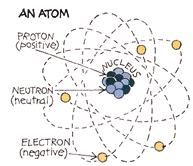
\includegraphics[width=1.0in]{atom.jpg},\centerline{The Atom}] The \verb+multicols+ package allows using multiple columns without starting a new page.  Using floats is not possible in a columns environment, however with the \verb+picinpar+ package, I can set a picture inside a block of text---just like you one you see here.  Isn't \LaTeX{} cool?
And now we're just filling more space, and yet more space.  
\end{window}
\closearticle


\headline{\it\huge Another Headline}
This is just an example to fill up some space, but as long as I have your attention, I'll give some newspaper advice.

It's good to use different fonts for each headline.  This particular font was accomplished with the command \verb+\headline{\it\huge Another Headline}+.  The headline in the preceding article was accomplished with the command \verb+\byline{\sc\Large Geek Designs New \LaTeX{} Package}{Matthew Allen}+.

Of course the commands don't look so nice when they're set in column format.  Look at the example file if you have any questions as to how this example was created.

I suppose we could also show how an equation is type set:
\begin{displaymath}
x=\frac{-b\pm\sqrt{b^2-4ac}}{2a}
\end{displaymath}
and there you have it.  \closearticle
}
\end{multicols}

\end{document}
